\documentclass{fkssolpub}

\usepackage[czech]{babel}
\usepackage{fontspec}
\usepackage{fkssugar}
\usepackage{amsmath}
\usepackage{graphicx}

\newcommand{\dd}{\mathrm{d}}
\renewcommand{\angle}{\sphericalangle}

\author{Ondřej Sedláček}
\school{Gymnázium Oty Pavla} 
\series{4}
\problem{2} 

\begin{document}

\begin{figure}
  \begin{center}
    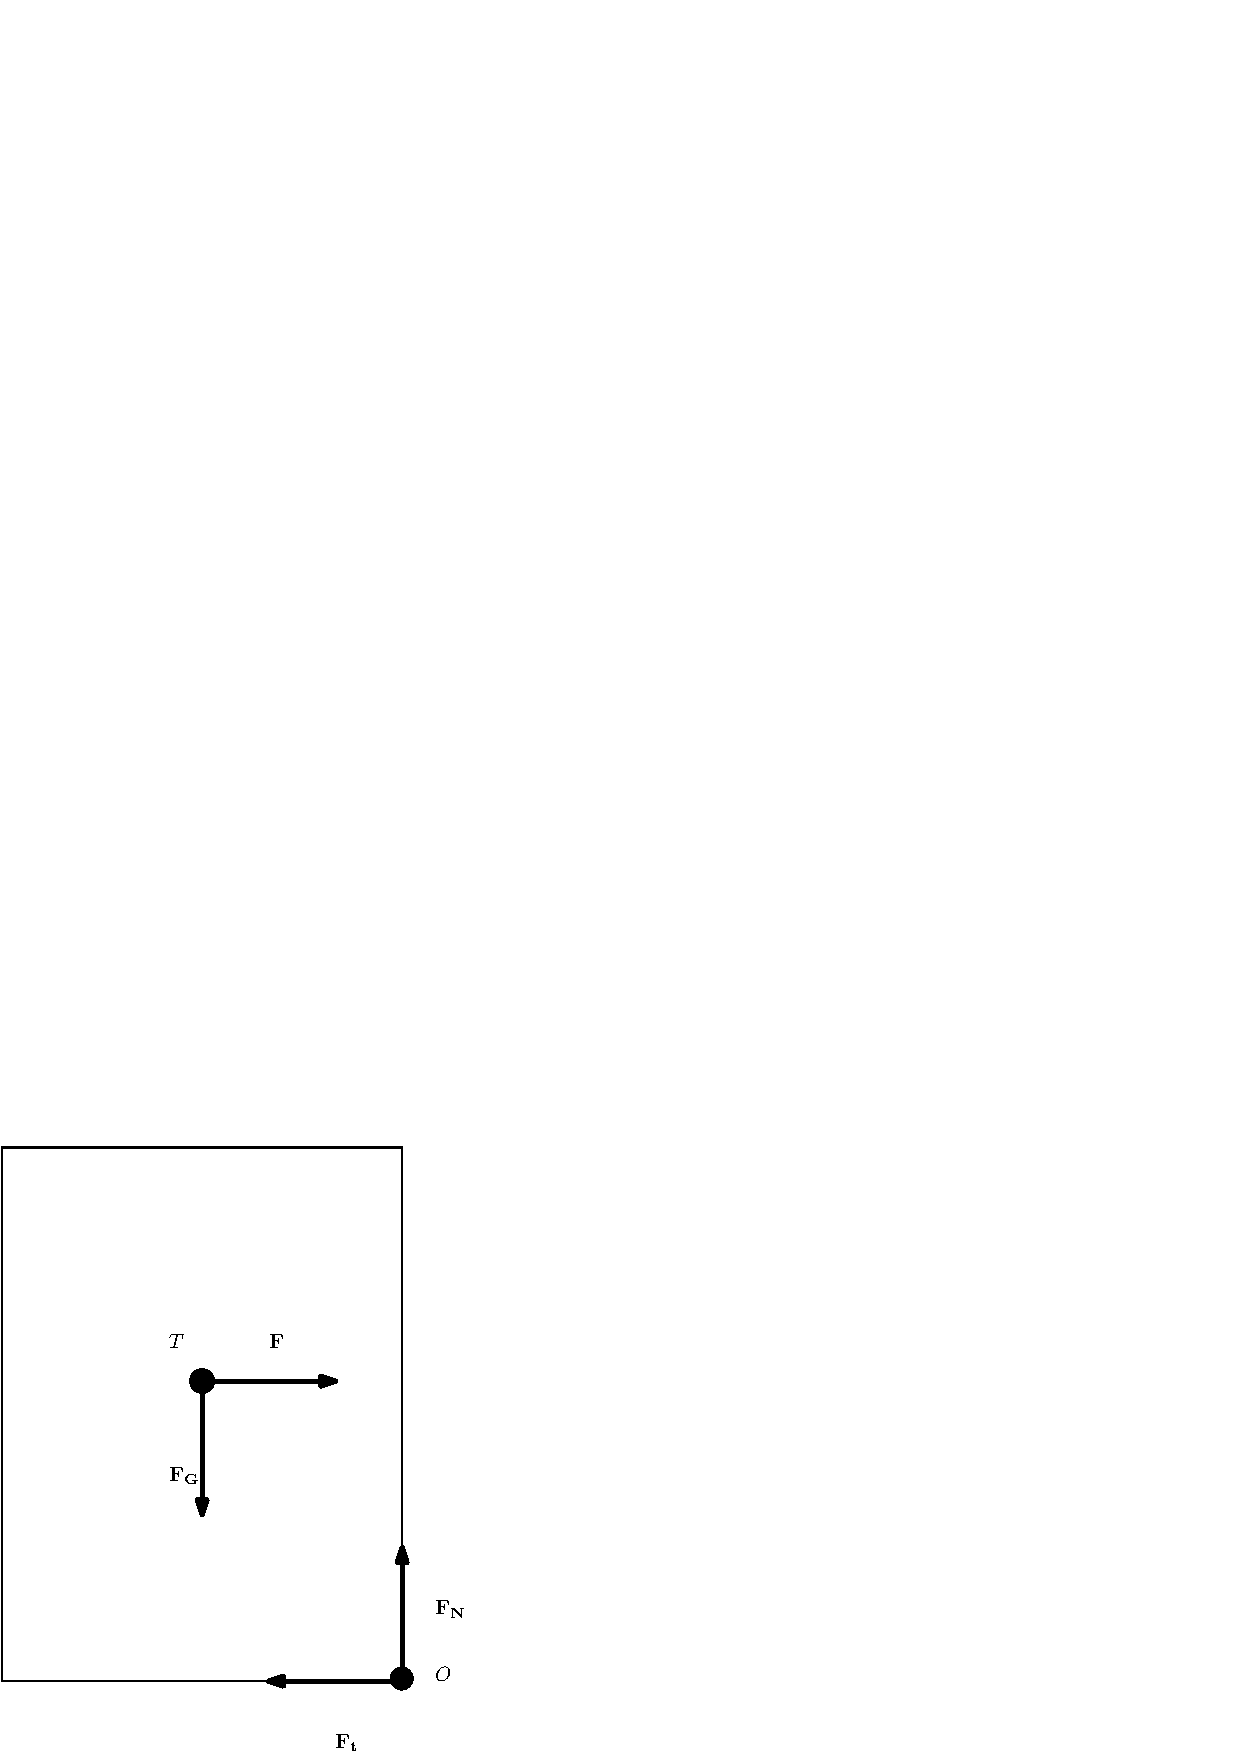
\includegraphics[width=0.95\textwidth]{2-fig.png}
  \end{center}
  \caption{Konstrukce k vysvětlení důkazu a značení}
  \label{fig:}
\end{figure}


Když se podíváme na trojúhelník $ACE$, můžeme si všimnout toho, že body $B$, $D$, $F$ jsou Švrčkovy body ke stranám $AC$, $CE$, $EA$, protože leží na osách těchto stran. Z toho tedy plyne, že tyto body zároveň leží na osách úhlů tohoto trojúhelníku, tedy přímky $AD$, $BE$ a $CF$ jsou osy úhlu trojúhelníku $ABE$, které procházejí vepsištěm tohoto trojúhelníku. Tím je tvrzení ze zadání dokázáno. Q. E. D.

\end{document}
